\chapter[Fermat's Last Theorem and Thorin Measures]{Weight One Forms, Wiles's Theorem\\ and Fermat: Is There a Thorin\\ Measure Form of Fermat's Last Theorem?}\label{ch:flt}

Two kinds of ``one forms'' carry the proof of Fermat's last theorem. Weight one modular forms enter through the Langlands Tunnell theorem, which makes the mod $3$ representation of a semistable elliptic curve modular when it is irreducible, and so starts Wiles's argument. Weight two forms are holomorphic differential $1$ forms $f(z)\,dz$ on the modular curve $X_0(N)$, and the proof ends with the fact that $X_0(2)$ has none. This chapter reads both through the probabilistic language of Chapters~\ref{ch:recip} and \ref{ch:hit}, and answers the question in the title. No step of the proof is reproved here, and no new case of modularity is proved.

Weight one newforms are exactly the newforms whose Frobenius label law is atomic (Proposition~\ref{prop:fltatomic}). The congruence of Wilton, which says that $\tau(p)$ is congruent modulo $23$ to the $p$th coefficient of $\eta(z)\eta(23z)$, and which we verify at all $25996$ primes $p<3\cdot10^5$, $p\ne23$, is a classical instance of the congruences between forms of different weights that Wiles needed. Modularity implies a symmetry in law: for $11a1$, whose form is $\eta(z)^2\eta(11z)^2$, the P\'olya kernel is a positive multiple of a probability density, and modularity (here Eichler and Shimura) makes the corresponding random variable symmetric; at this level, given the Euler product, the symmetry also implies modularity, by a converse theorem of Conrey and Farmer. For $37a1$ the kernel is odd and the root number is $-1$ (Proposition~\ref{prop:fltsymmetric}). An elliptic curve carries three Thorin objects: the Thorin measure of its Frobenius functionals, the unconditional Rankin Selberg generalized gamma convolution, and the counting measure of its squared zeros, which is positive exactly under GRH. We compute the heat trace of $11a1$ from its point counts modulo primes, its conductor and its gamma factor, matching the sum over its zeros to a relative error below $2\cdot10^{-13}$, and its integral over $x\ge e^{-60}$, $0.127589010327$, against $\frac12\sum\gamma^{-2}=0.127589010329$, summed over all zeros, from the Hadamard product. Under GRH this constant is the mean explosion time of the birth process of Chapter~\ref{ch:hit} whose rates are the squared ordinates of the zeros, and that explosion time and the P\'olya variable form an explicit Wald couple (Proposition~\ref{prop:fltwald}).

The answer to the title question has three parts. There is no Thorin measure statement equivalent to Fermat's last theorem in a meaningful sense: Fermat is a statement about rational points, Thorin measures see $L$ functions, and the bridge used in the proof is modularity. What does exist is a Thorin form of the last step. Attach to each prime level $N$ and auxiliary prime $\ell$ the generalized gamma convolution whose Thorin atoms are the numbers $\ell+1-a_\ell(f)$ for the weight two newforms $f$ of level $N$. Its Thorin measure is empty exactly when $X_0(N)$ has genus zero, when there is one supersingular elliptic curve in characteristic $N$, and when the isogeny walk of Chapter~\ref{ch:hit} has nowhere to go (Theorem~\ref{thm:fltempty}). The conclusion of Ribet's level lowering is the vanishing of a mod $p$ discrepancy Thorin mass (Proposition~\ref{prop:fltmodp}), illustrated by a newform of level $77$ congruent to $11a1$ modulo $3$ at all $2259$ primes tested. Given the theorems of Wiles, Taylor and Wiles, Ribet and Mazur, Fermat's last theorem for prime exponents $p\ge5$ follows from the emptiness of the level $2$ Thorin measure (Theorem~\ref{thm:fltflt}), which is the class number one of the Hurwitz quaternions. Section~\ref{sec:fltexplicit} makes the connection explicit. The Frobenius functional that counts primes $\ell$ with $p\nmid|E(\mathbb F_\ell)|$ converges to a Gamma law whose shape $c(E,p)$, a local density of Koblitz's conjecture \cite{koblitz1988,zywina2011}, we call the Eisenstein Thorin shape; it equals $1-(p^2-2)/((p^2-1)(p-1))$ when the image is $\GL_2(\mathbb F_p)$, and it vanishes exactly when $\bar\rho_{E,p}$ is Eisenstein (Proposition~\ref{prop:flteisgamma}). By Serre's argument from Mazur's torsion theorem, a Frey curve has $c(E,p)>0$ for $p\ge5$, while its rational $2$ torsion forces $c(E,2)=0$ (Proposition~\ref{prop:flteisfrey}); the Frey type curve of $3+5^3=2^7$ has measured shapes $0,0,0.762,0.837$ at $p=2,3,5,7$ over the primes $\ell<2\cdot10^6$, against $73/96=0.760$ and $241/288=0.837$ for image $\GL_2(\mathbb F_p)$. Given the same theorems, Fermat's last theorem is the incompatibility of two Thorin statements: a positive Eisenstein shape and an empty cuspidal Thorin measure at level $2$ (Theorem~\ref{thm:flttwo}). The deep content is in the theorems of Langlands and Tunnell, Wiles, Taylor and Wiles, Ribet and Mazur, not in the probabilistic restatement.

\section{The architecture of the proof}\label{sec:fltproof}

Fermat's last theorem asserts that $a^n+b^n=c^n$ has no solution in nonzero integers for $n\ge3$. Its proof, completed by Wiles \cite{wiles1995} with Taylor and Wiles \cite{taylorwiles1995}, runs through a chain of reductions due to Hellegouarch, Frey, Serre and Ribet \cite{hellegouarch1975,frey1986,serre1987,ribet1990}. It suffices to treat $n=4$, done by Fermat, and odd primes $n=p$, the case $p=3$ being Euler's. In outline: a solution with $n=p\ge5$ prime produces a semistable elliptic curve $E$, the Frey curve; $E$ is modular by Theorem~\ref{thm:fltwiles}; Ribet's theorem then forces the mod $p$ Galois representation of $E$ to come from a weight two newform of level $2$; and there are no such forms, because the modular curve $X_0(2)$ has genus zero.

Suppose $a^p+b^p=c^p$ with $abc\ne0$, $p\ge5$ prime, $\gcd(a,b,c)=1$, and after permuting and changing signs $a\equiv-1\bmod4$ and $b$ even. The Frey curve
\[E:\ y^2=x(x-a^p)(x+b^p)\]
is semistable \cite{frey1986,serre1987}. Its conductor is the product $N_E$ of the primes dividing $abc$, and its minimal discriminant is $2^{-8}(abc)^{2p}$. Its mod $p$ representation\[\bar\rho_{E,p}:\Gal(\overline\Q/\Q)\to\GL_2(\mathbb F_p)\]is irreducible, by Serre's argument \cite{serre1987} from Mazur's torsion theorem \cite{mazur1977}, since $E$ is semistable with all its $2$ torsion rational \cite[Theorem~2.9(c)]{ddt1995}. It is unramified at every odd prime $q\ne p$ of multiplicative reduction, because the exponent of $q$ in the minimal discriminant is divisible by $p$, and it is finite flat at $p$, by the same divisibility if $p\mid abc$ and because $E$ has good reduction at $p$ otherwise. At $2$ the exponent $2pv_2(b)-8$ of the minimal discriminant is not divisible by $p$, so $\bar\rho_{E,p}$ is ramified at $2$.

\begin{theorem}[Wiles; Taylor and Wiles \cite{wiles1995,taylorwiles1995}]\label{thm:fltwiles}
Every semistable elliptic curve over $\Q$ is modular: there is a weight two newform $f$ of level $N_E$ with $a_\ell(f)=\ell+1-|E(\mathbb F_\ell)|$ for all $\ell\nmid N_E$.
\end{theorem}

Breuil, Conrad, Diamond and Taylor \cite{bcdt2001} removed the semistability hypothesis (Theorem~\ref{thm:02modularity}).

\begin{theorem}[Ribet \cite{ribet1990}, Theorem~1.1; see \cite{ddt1995}]\label{thm:fltribet}
Let $p$ be an odd prime, $f$ a weight two newform of level $N$ with trivial character, $\mathfrak p$ a prime above $p$ of its coefficient field with $\bar\rho_{f,\mathfrak p}$ irreducible, and $q\| N$ a prime at which $\bar\rho_{f,\mathfrak p}$ is unramified, or finite flat if $q=p$. If $q\not\equiv1\bmod p$ or $p\nmid N$, there are a weight two newform $g$ of level dividing $N/q$ with trivial character and a prime $\mathfrak p'$ above $p$ of its coefficient field with $\bar\rho_{g,\mathfrak p'}\cong\bar\rho_{f,\mathfrak p}$ over $\overline{\mathbb F}_p$.
\end{theorem}

Applied to the Frey curve, first at $q=p$ if $p\mid N_E$, where $q\not\equiv1\bmod p$ holds trivially, and then one at a time at the odd primes $q\ne p$ of the level, which is now prime to $p$, Theorems~\ref{thm:fltwiles} and \ref{thm:fltribet} give a weight two newform of level dividing $2$. There is none, since $S_2(\Gamma_0(1))=0$ and $\dim S_2(\Gamma_0(2))$ is the genus of $X_0(2)$, which is $0$. This is the whole skeleton; the depth is in Theorems~\ref{thm:fltwiles} and \ref{thm:fltribet} and in Mazur's torsion theorem.

\section{Weight one forms}\label{sec:fltweightone}

A newform $f$ of weight one and level $N$ gives, by Deligne and Serre \cite{deligneserre1974}, an odd irreducible two dimensional Artin representation $\rho$ with $\tr\rho(\Frob_p)=a_p(f)$ for $p\nmid N$; its character is $\det\rho$. The image of $\rho$ is finite, its projective image is dihedral, $A_4$, $S_4$ or $A_5$, and the Ramanujan bound $|a_p|\le2$ holds trivially. Conversely every odd irreducible two dimensional Artin representation arises in this way, by Hecke, Langlands and Tunnell \cite{langlands1980,tunnell1981} when the projective image is solvable, and in general by Khare and Wintenberger \cite{kharewintenberger2009,kharewintenberger2009b}, with work of Kisin \cite{kisin2009}. The book's running example (Example~\ref{ex:ch3cubic}) is $\eta(z)\eta(23z)$, of level $23$ and character $(\frac{-23}\cdot)$, attached to the $S_3$ representation of the splitting field of $x^3-x-1$: $a_p=2,0,-1$ as $x^3-x-1$ has $3$, $1$ or $0$ roots modulo $p$, for $p\ne23$.

\subsection{Weight one forms in Wiles's proof}

Wiles's argument starts from a modular residual representation. Suppose that $\bar\rho_{E,3}$ is irreducible. Its image lies in $\GL_2(\mathbb F_3)$, which is solvable, and $\GL_2(\mathbb F_3)$ embeds in $\GL_2(\Z[\sqrt{-2}])$ compatibly with reduction modulo $1+\sqrt{-2}$. Composing gives an odd Artin representation with octahedral or smaller projective image, which by Langlands and Tunnell \cite{langlands1980,tunnell1981} comes from a weight one form $g$. The character of $g$ is $\chi_{-3}=(\frac{-3}\cdot)$, which lifts $\det\bar\rho_{E,3}$. Multiplying $g$ by the weight one Eisenstein series $E_{1,\chi_{-3}}$, the theta series of $x^2+xy+y^2$, which is congruent to $1$ modulo $3$, gives a weight two form with trivial character congruent to $g$, and the lemma of Deligne and Serre \cite{deligneserre1974} gives a weight two eigenform with the same congruence, so $\bar\rho_{E,3}$ is modular of weight two \cite{wiles1995,ddt1995}. When $\bar\rho_{E,3}$ is reducible, which for semistable $E$ is the same as reducibility of its restriction to $\Gal(\overline\Q/\Q(\sqrt{-3}))$ \cite{ddt1995}, Wiles passes to $p=5$ through an auxiliary curve, the $3$ to $5$ switch. So a weight one form, and through it the Langlands Tunnell theorem for solvable groups, is the base of the proof.

The mechanism, a weight one form congruent to a form of higher weight, has a classical prototype. Wilton \cite{wilton1930} proved, and Serre \cite{serre1968b} explained through the mod $23$ representation of $\Delta$ (see also Swinnerton Dyer \cite{swinnertondyer1973}), that Ramanujan's $\tau$ is controlled modulo $23$ by the $S_3$ field of $x^3-x-1$:
\[
\tau(p)\equiv a_p\bigl(\eta(z)\eta(23z)\bigr)\pmod{23}\qquad(p\ne23),
\]
so $\tau(p)\equiv0$, $2$ or $-1$ modulo $23$ according as $p$ is inert in $\Q(\sqrt{-23})$, splits completely in the $S_3$ field, or neither. Equivalently, the mod $23$ representation of $\Delta$ is the reduction of the $S_3$ representation, so its projective image is $S_3$, and away from $23$ the weight $12$ form $\Delta$ is congruent to the weight one form $\eta(z)\eta(23z)$. We checked the congruence at all $25996$ primes $p<3\cdot10^5$, $p\ne23$, with no exception.

\subsection{Weight one is an atomic label law}

In the Gamma process of Section~\ref{sec:recipgammaproc} the prime factors of a zeta random integer carry labels, here the normalised coefficients $x_p=a_p(f)/p^{(k-1)/2}$ of a newform $f$ of weight $k$. The label law $\mu_f$ is the limit of their empirical distribution.

\begin{proposition}[atomic labels characterise weight one]\label{prop:fltatomic}
For a newform $f$ of weight $k\ge1$ the following are equivalent: (i) $k=1$; (ii) $x_p$ takes finitely many values; (iii) the label law $\mu_f$ is finitely supported. In that case $\mu_f$ is the image of Haar measure on the finite image of the Deligne Serre representation under the trace.
\end{proposition}

\begin{proof}
If $k=1$, Deligne and Serre give a finite image $G$, so $x_p=\tr\rho(\Frob_p)$ takes finitely many values and Chebotarev gives $\mu_f$ as the image of Haar measure on $G$. If $k\ge2$ and $f$ has complex multiplication, Hecke's theorem gives $\mu_f=\mu_{\mathrm{CM}}=\frac12\delta_0+\frac12\nu$ (Section~\ref{sec:04cm}), with $\nu$ the continuous law of $2\cos\theta$, $\theta$ uniform; if $f$ has no complex multiplication and trivial character, $\mu_f$ is the semicircle law by the Sato Tate theorem \cite{blght2011}. With a character $\psi$, $x_p/\zeta$ is equidistributed for the semicircle law on the primes with $\psi(p)=\zeta^2$ \cite[Theorem~B]{blght2011}, so $\mu_f$ is a mixture of rotated semicircle laws, and with complex multiplication the law above is rotated in the same way. None of these laws is finitely supported, and in every case $x_p$ takes infinitely many values.
\end{proof}

Figure~\ref{fig:fltlabels} shows the two kinds of label law. Among the primes $p\ne23$ below $2\cdot10^5$ the coefficients of $\eta(z)\eta(23z)$ take the values $-1,0,2$ with frequencies $0.334,0.502,0.165$ (and $0.33336,0.50027,0.16637$ below $10^7$, Example~\ref{ex:ch3cubic}), against Haar measure $\frac13,\frac12,\frac16$ on $S_3$, while $a_p/\sqrt p$ for the weight two form of $11a1$ follows the semicircle. In Thorin terms a Frobenius functional of a weight one form is a finite gamma convolution with atomic Thorin measure (Theorem~\ref{thm:recipggcfun} with a finite label space), while for weight two and $Q(x)=x^2$ (Figure~\ref{fig:fltkernels}, right) it is a generalized gamma convolution with a continuous Thorin measure.

\begin{figure}[t]
\centering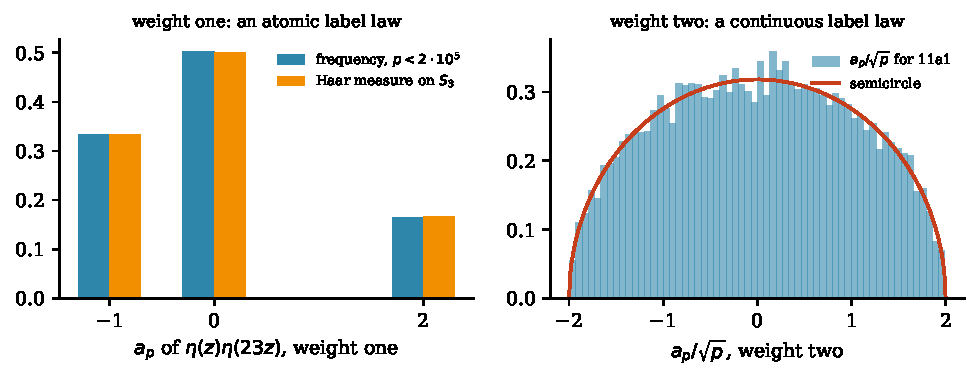
\includegraphics[width=\textwidth]{figs/flt_labels.pdf}
\caption{Proposition~\ref{prop:fltatomic}. Left: the coefficients of the weight one form $\eta(z)\eta(23z)$ over primes below $2\cdot10^5$, against Haar measure on $S_3$. Right: the normalised coefficients of the weight two form of $11a1$, against the semicircle.}\label{fig:fltlabels}
\end{figure}

\section{Modularity and symmetry in law}\label{sec:fltsymmetry}

Let $E$ have conductor $N$ and $L$ series $\sum a_nn^{-s}$, and put $f(z)=\sum a_ne^{2\pi inz}$. The P\'olya kernel of Chapter~\ref{ch:recip},
\[
\Phi_E(u)=f\Bigl(\frac{ie^u}{\sqrt N}\Bigr)e^{u},\qquad \Lambda(1+t,E)=\int_{\R}\Phi_E(u)e^{tu}\,du,
\]
with $\Lambda(s,E)=N^{s/2}(2\pi)^{-s}\Gamma(s)L(s,E)$, is built from the point counts $a_p=p+1-|E(\mathbb F_p)|$ and the conductor. By Hecke's criterion (Proposition~\ref{prop:recipsym}), $f$ satisfies the Fricke transformation with root number $\varepsilon$ if and only if $\Phi_E(-u)=\varepsilon\,\Phi_E(u)$. Weil's converse theorem \cite{weil1967} upgrades the corresponding reflection identities for the twisted kernels $\Phi_{E\otimes\chi}$, which pair $\chi$ with $\bar\chi$ and are complex valued, to modularity; Problem~\ref{cp:recipkernel} poses their numerical test. For $11a1$ the reflection of $\Phi_E$ alone suffices, given the Euler product: the converse theorem of Conrey and Farmer \cite{conreyfarmer1995} replaces the twists by the shape of the Euler factors at the levels $5\le N\le12$, $14\le N\le17$ and $23$. So Theorem~\ref{thm:fltwiles} says, for a semistable $E$, that a family of functions built from point counts and the conductor has the reflection symmetries of a modular form.

\begin{proposition}[the P\'olya variable of an elliptic curve; after Proposition~\ref{prop:recipsym}]\label{prop:fltsymmetric}
Let $f$ be the newform of an elliptic curve $E$ and suppose $\Phi_E\ge0$. Then $\Phi_E/\Lambda(1,E)$ is the density of a random variable $W_E$ with $\E e^{tW_E}=\Lambda(1+t,E)/\Lambda(1,E)$ for all real $t$, and $W_E$ is symmetric in law; positivity forces the root number to be $+1$, since a kernel with $\varepsilon=-1$ is odd. For $E=11a1$, $f(z)=\eta(z)^2\eta(11z)^2$ is positive on the imaginary axis, so $W_E$ exists and is symmetric.
\end{proposition}

\begin{proof}
The Mellin formula gives the transform, which converges for all real $t$ because $f(iy)$ decays exponentially as $y\to\infty$ and, by the Fricke symmetry, as $y\to0$. Symmetry is Hecke's criterion with $\varepsilon=+1$. The product formula $\eta(z)=q^{1/24}\prod(1-q^n)$ is positive on $z=iy$, and the root number of $11a1$ is $+1$.
\end{proof}

We computed $\Phi_E$ from the first $4000$ coefficients for $11a1$ and $37a1$ (Figure~\ref{fig:fltkernels}, left). For $11a1$ the kernel is positive, with minimum $1.2\cdot10^{-9}$ on $|u|\le2.5$, and $\max|\Phi_E(u)-\Phi_E(-u)|=9\cdot10^{-17}$. For $37a1$, the curve of smallest conductor with positive rank, the root number is $-1$ and the kernel is odd to $4\cdot10^{-16}$: the parity of the analytic rank is the parity of a P\'olya kernel. A Frey curve, if it existed, would by Theorem~\ref{thm:fltwiles} have kernels with all the twisted reflection symmetries; by Ribet its mod $p$ labels would agree with those of a level $2$ form; there is none.

\begin{figure}[t]
\centering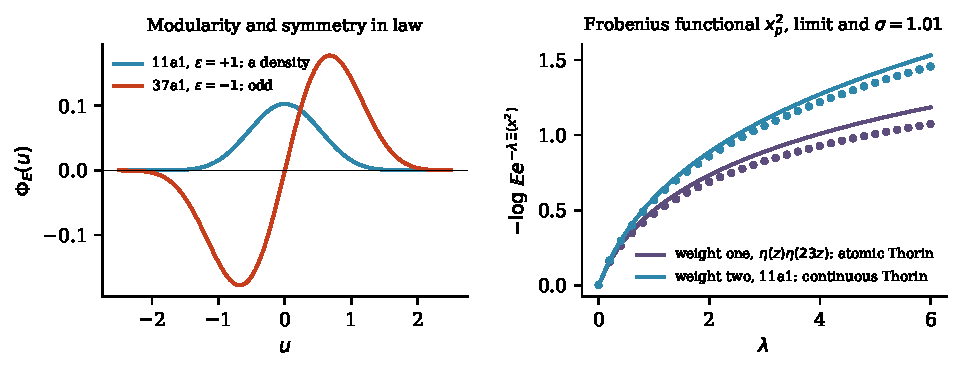
\includegraphics[width=\textwidth]{figs/flt_kernels.pdf}
\caption{Left: P\'olya kernels $\Phi_E(u)$ (solid) and $\varepsilon\Phi_E(-u)$ (dashed, hidden under the solid curves) computed from point counts and the conductor: $11a1$, a positive multiple of a symmetric probability density, and $37a1$, odd. Right: the Frobenius functional $\Xi_\sigma(Q)$, $Q(x)=x^2$, of the zeta random integer for the weight one form $\eta(z)\eta(23z)$ and the weight two form of $11a1$, shown as $-\log\E e^{-\lambda\,\Xi_\sigma(Q)}$: the limits $\int\log(1+\lambda x^2)\,d\mu$ (lines) and the values at $\sigma=1.01$ from the Euler product over the primes below $10^7$, the rest estimated by the prime number theorem (dots). Both have mean $1$; their Thorin measures differ.}\label{fig:fltkernels}
\end{figure}

\section{The Thorin measures of an elliptic curve}\label{sec:fltthorinec}

For an elliptic curve, or any weight two newform, there are three Thorin objects, of increasing depth.

\emph{Frobenius functionals.} By Theorem~\ref{thm:recipggcfun} the functional $\Xi_\sigma(Q)$ of the zeta random integer, with labels $x_p=a_p/\sqrt p$, converges to the GGC whose Thorin measure is the image of the label law, restricted to $\{Q>0\}$, under $x\mapsto1/Q(x)$. For $Q(x)=x^2$ and $11a1$ this is the law of $1/X^2$ for $X$ semicircular, a continuous Thorin measure; for the weight one form $\eta(z)\eta(23z)$ it is atomic, $\frac16\delta_{1/4}+\frac13\delta_1$. Both GGCs have mean $\int x^2\,d\mu=1$, which is the orthonormality of Theorem~\ref{thm:recipcusp} in the form \emph{unit second moment}; the Thorin measures, images of the label laws, are what distinguish weight one from weight two (Figure~\ref{fig:fltkernels}, right; Proposition~\ref{prop:fltatomic}). These statements are unconditional.

\emph{The Rankin Selberg GGC.} Let $D(s)$ be the Rankin Selberg Euler product of $E$ in the unitary normalisation, with $\alpha_p=a_p/\sqrt p$ and $\beta_p=0$ at the primes $p\mid N$, so that $-D'/D(s)=\sum_{p,m}|\alpha_p^m+\beta_p^m|^2(\log p)p^{-ms}$ with nonnegative coefficients and $D$ has a pole at $s=1$; for semistable $E$, $D$ is $L(s,E\times E)$ without its factors $(1-p^{-s})^{-1}$ at the primes $p\mid N$. For $\alpha>1$ put
\[
U_\alpha(z)=\frac1{2\pi\sqrt z}\sum_{p,m}|\alpha_p^m+\beta_p^m|^2(\log p)\,p^{-m\alpha}\,2\sin^2\Bigl(\frac{m\log p\,\sqrt z}2\Bigr).
\]
By Lemma~\ref{lem:10dsin2} with $f=D$, as for the density $U_{\mathrm{ar}}$ of Section~\ref{sec:10daway} (Proposition~\ref{prop:recipfamily} is the analogue for Artin representations),
\[
e^{\sqrt s\,D'/D(\alpha)}\,\frac{D(\alpha)}{D(\alpha+\sqrt s)}
\]
is the Laplace transform of a GGC with Thorin density $U_\alpha$. It is computed from point counts and is positive unconditionally. Figure~\ref{fig:fltthorinec}, right, shows $U_\alpha$ for $11a1$ at $\alpha=1.5$ and $1.2$, with the bad prime $11$ entering through $|\alpha_{11}^m|^2=11^{-m}$; it grows as $\alpha$ decreases towards the pole at $s=1$.

\emph{The zeros.} The deepest object is the Galois heat trace $\mathcal W_E$ of Definition~\ref{def:recipheat}, given by the explicit formula from the point counts, the conductor and the gamma factor. Since $L(s,E)$ is entire by modularity (Theorem~\ref{thm:02modularity}), Theorem~\ref{thm:recipcm} gives $\mathcal W_E(x)=\frac12\sum e^{-x\gamma^2}$, the sum over the zeros $1+i\gamma$ of $\Lambda(s,E)$ with multiplicity, which are the zeros $\frac12+i\gamma$ in the unitary normalisation of Chapter~\ref{ch:recip}, and $\mathcal W_E$ is completely monotone if and only if GRH holds for $L(s,E)$. Its Bernstein measure is then $\frac r2\delta_0+\sum_{\gamma>0}\delta_{\gamma^2}$, where $r$ is the order of the zero at the centre, which is odd when the root number is $-1$; for $11a1$, $r=0$. If $r=0$ and GRH holds, Theorem~\ref{thm:hitexplosion} makes $\mathcal W_E(x)/x$ the L\'evy density of the explosion time $T_E$ of a pure birth process with rates $\gamma^2$, with $\E T_E=\int_0^\infty\mathcal W_E(x)\,dx=\sum_{\gamma>0}\gamma^{-2}$; by the same theorem $T_E$ exists only if GRH holds for $L(s,E)$, which is not known.

For $11a1$ we computed $\mathcal W_E$, as Chapter~\ref{ch:hit} does for the $S_3$ representation, from the conductor $11$, the gamma factor and the point counts at the $664579$ primes below $10^7$ and their powers, with the bad prime $11$ entering through $a_{11}=1$. It agrees with the sum over the zeros to fifteen digits at $x=0.002$, $0.01$ and $0.05$ and to thirteen digits at $x=0.2$ (Figure~\ref{fig:fltthorinec}, left), finite differences give its first two derivatives the signs required by complete monotonicity at $x=0.05,0.1,0.2,0.4$, and
\[
\int_{e^{-60}}^{2}\mathcal W_E(x)\,dx=0.127589010327
\]
from point counts, against $0.127589010329$ computed by PARI for $\frac12\sum\gamma^{-2}=\frac12\Lambda''(1,E)/\Lambda(1,E)$, an identity of the Hadamard product that needs no hypothesis; this is the constant $S_1$ of $11a1$ in Table~\ref{tab:10bcatalogue}. The first zero is $\gamma_1=6.3626$, so $\mathcal W_E(x)<e^{-80}$ for $x\ge2$, and the difference $1.6\cdot10^{-12}$ is the part of the integral over $x<e^{-60}$, which the quadrature leaves out and which the density of the zeros gives as $1.55\cdot10^{-12}$; with it the two values differ by $6\cdot10^{-17}$. As in Chapter~\ref{ch:hit}, the agreement does not verify GRH: a finite computation of this kind can disprove it and is not known to verify it.

\begin{proposition}[an explicit Wald couple; after Theorem~\ref{thm:10dvdp}]\label{prop:fltwald}
Assume GRH for $L(s,11a1)$. Then the P\'olya variable $W_E$ of Proposition~\ref{prop:fltsymmetric} and the explosion time $T_E$ satisfy\[\E e^{tW_E}\,\E e^{-t^2T_E}=1\qquad\text{for every real }t:\]they form a Wald couple in the sense of Definition~\ref{def:10dwald}, built respectively from the modular form $\eta(z)^2\eta(11z)^2$ and from the zeros of its $L$ function.
\end{proposition}

\begin{proof}
This is the implication from (a) to (c) of Theorem~\ref{thm:10dvdp} for $\eta(z)^2\eta(11z)^2$, with $Z_\pi=T_E$. Directly: $\E e^{tW_E}=\Lambda(1+t,E)/\Lambda(1,E)$, and under GRH
\[
\E e^{-t^2T_E}=\prod_{\gamma>0}\Bigl(1+\frac{t^2}{\gamma^2}\Bigr)^{-1}=\frac{\Lambda(1,E)}{\Lambda(1+t,E)}
\]
by the Hadamard product, since $\Lambda(1,E)\ne0$ and $\Lambda(1+z,E)$ is even of order one, so its exponential factors cancel in pairs.
\end{proof}

\begin{figure}[t]
\centering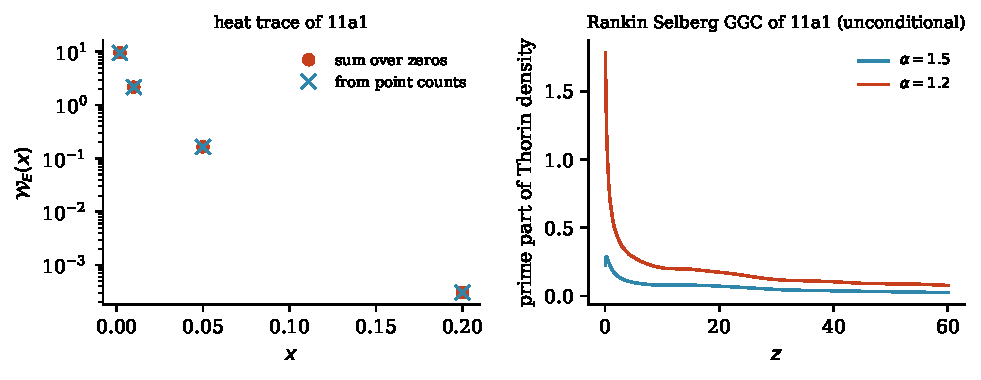
\includegraphics[width=\textwidth]{figs/flt_thorin.pdf}
\caption{Left: the heat trace of $11a1$ computed from the point counts modulo the primes below $10^7$, the conductor and the gamma factor (crosses), against the sum over its zeros (dots). Right: the Rankin Selberg Thorin density $U_\alpha$ of $11a1$ at $\alpha=1.5$ and $1.2$, positive unconditionally, summed over the primes below $10^7$; the larger primes would add under $0.4$ percent at $\alpha=1.5$ and between $3.5$ and $9.3$ percent at $\alpha=1.2$.}\label{fig:fltthorinec}
\end{figure}

\section{Weight two forms are one forms}\label{sec:fltoneforms}

For $f\in S_2(\Gamma_0(N))$ the differential $f(z)\,dz$ is invariant under $\Gamma_0(N)$ and holomorphic at the cusps, and every holomorphic $1$ form on $X_0(N)$ arises this way, so $\dim S_2(\Gamma_0(N))=g(X_0(N))$. For prime $N$, by Deuring \cite{deuring1941} and Eichler, the number of supersingular elliptic curves over $\overline{\mathbb F}_N$ is $g(X_0(N))+1$, and by Eichler and Gross the $1$ forms on $X_0(N)$ correspond to the nonconstant eigenfunctions of the isogeny walk of Section~\ref{sec:hitisogeny} \cite{eichler1954,eichler1973,gross1987} (Theorem~\ref{thm:08brandt} for $N\equiv1\bmod12$). The genus is zero exactly for $N\in\{2,3,5,7,13\}$ among primes; PARI/GP gives $\dim S_2(\Gamma_0(N))=0,0,0,0,1,0,1,1,2$ for $N=2,3,5,7,11,13,17,19,23$.

At $N=2$ there is one supersingular curve, $j=0=1728$ in characteristic $2$, with automorphism group of order $24$; with $w=|\operatorname{Aut}E|/2=12$, Eichler's mass formula $\sum1/w=(N-1)/12$ of Chapter~\ref{ch:hit} reads $1/12=1/12$. Its endomorphism ring is the Hurwitz order of quaternions $\frac12(a+bi+cj+dk)$ with $a,b,c,d$ all even or all odd, which has class number one. The theta series of its norm form lies in $M_2(\Gamma_0(2))$, which is spanned by an Eisenstein series because $S_2(\Gamma_0(2))=0$, and so counts exactly: the number of Hurwitz quaternions of norm $n$ is $24\sum_{d\mid n,\,d\text{ odd}}d$. We checked this by enumeration for $n\le60$; the first values are $24,24,96,24,144,96,192,24$. The isogeny walk has a single state, and every $\ell$ isogeny returns to the same curve.

\section{Is there a Thorin measure form of Fermat's last theorem?}\label{sec:fltthorin}

The answer has three parts.

First, no Thorin statement is \emph{equivalent} to Fermat's last theorem in a useful sense. Fermat is about rational points on the curves $x^p+y^p=1$; Thorin measures are attached to $L$ functions and Frobenius statistics. The bridge used in the proof, and the only one known for all exponents, is modularity, a deep theorem. Any true statement is formally equivalent to any other, so the question is what Fermat \emph{reduces to}, after the deep theorems.

Second, it reduces to the emptiness of a Thorin measure.

\begin{definition}\label{def:flthecke}
For a prime $N$ and a prime $\ell\ne N$, the \emph{Hecke GGC} $H_N(\ell)$ is the generalized gamma convolution with Thorin measure $\sum_f\delta_{\ell+1-a_\ell(f)}$, the sum over the normalised eigenforms of $S_2(\Gamma_0(N))$.
\end{definition}

The atoms are positive because $a_\ell(f)<\ell+1$, which Perron Frobenius gives on the connected supersingular isogeny graph (the bound $|a_\ell(f)|\le2\sqrt\ell$ of Eichler and Shimura with Weil, as in Chapter~\ref{ch:hit}, gives more), so $H_N(\ell)$ is a sum of independent exponential variables with rates $\ell+1-a_\ell(f)$, the time that a pure birth chain with these rates takes to pass through its states. For a rational $f$ attached to an elliptic curve $E_f$ the rate is $|E_f(\mathbb F_\ell)|$. By \eqref{eq:hitjac} and Theorem~\ref{thm:hitkemeny},
\[
\E e^{-sH_N(\ell)}=\prod_f\frac{\ell+1-a_\ell(f)}{\ell+1+s-a_\ell(f)}=\frac{|J_0(N)(\mathbb F_\ell)|}{\det\bigl((\ell+1+s)-T_\ell\mid S_2(\Gamma_0(N))\bigr)},
\]
and $\E H_N(\ell)=K_N(\ell)/(\ell+1)$, with $K_N(\ell)$ the Kemeny constant of the supersingular $\ell$ isogeny walk in characteristic $N$. Chapter~\ref{ch:lap} inverts this transform through the B spline whose knots are the atoms $\ell+1-a_\ell(f)$ (Theorem~\ref{thm:lapspline}).

\begin{theorem}[empty Thorin measures]\label{thm:fltempty}
For a prime $N$ and a prime $\ell\ge5$, $\ell\ne N$, the following are equivalent.
\begin{enumerate}
\item[(a)] The curve $X_0(N)$ has genus zero, so it carries no nonzero holomorphic $1$ form and $S_2(\Gamma_0(N))=0$.
\item[(b)] The Thorin measure of $H_N(\ell)$ is zero, that is $H_N(\ell)=0$ almost surely.
\item[(c)] $|J_0(N)(\mathbb F_\ell)|=1$.
\item[(d)] There is exactly one supersingular elliptic curve over $\overline{\mathbb F}_N$, and the isogeny walk has a single state.
\item[(e)] The Kemeny constant $K_N(\ell)$ vanishes.
\end{enumerate}
\end{theorem}

\begin{proof}
(a) and (b) are the same statement, since the atoms are indexed by eigenforms. (a) implies (c) because $J_0(N)=0$. If $g\ge1$, the Weil bound gives $|J_0(N)(\mathbb F_\ell)|=\prod_f(\ell+1-a_\ell(f))\ge(\sqrt\ell-1)^{2g}$, as in Corollary~\ref{cor:hithasse}, and $(\sqrt5-1)^2>1$, so (c) implies (a). (a) is equivalent to (d) by the count $g+1$ of supersingular curves, and to (e) by Theorem~\ref{thm:hitkemeny}, which writes $K_N(\ell)$ as a sum of $g$ positive terms.
\end{proof}

Third, Ribet's theorem produces a newform whose mod $p$ discrepancy Thorin mass against the given one vanishes; equivalently, by Theorem~\ref{thm:hitrate}, the discrepancy set of primes is hit by the prime factors of a random integer at rate zero. Label the primes by the pair of mod $p$ Frobenius classes of two Galois representations; by Chebotarev these labels are equidistributed on a finite group, and Theorem~\ref{thm:recipggcfun} applies with a finite label space, as in Theorem~\ref{thm:recipthorin}(a) for Artin representations.

\begin{proposition}[mod $p$ reciprocity as a vanishing Thorin mass; compare Theorem~\ref{thm:recipthorin}(a)]\label{prop:fltmodp}
Let $\rho_1,\rho_2$ be the representations, at primes above $p$ of the coefficient fields, of two weight two newforms with trivial character, or of an elliptic curve and such a newform, with semisimple reductions $\bar\rho_1,\bar\rho_2$ over a common finite field $k$ of characteristic $p$. Let $D_p$ be the set of primes $\ell\nmid pN_1N_2$ with $\tr\bar\rho_1(\Frob_\ell)\ne\tr\bar\rho_2(\Frob_\ell)$ in $k$, and $Q=\mathsf 1_{D_p}$. The following are equivalent: (i) $\bar\rho_1\cong\bar\rho_2$; (ii) $D_p$ has Dirichlet density zero; (iii) the Frobenius functional $\Xi_\sigma(Q)$ of the zeta random integer converges to $0$, its Thorin measure being zero.
\end{proposition}

\begin{proof}
Both representations factor through the finite group $G=\Gal(K/\Q)$ cut out by $\bar\rho_1\oplus\bar\rho_2$, and $D_p$ is the set of primes whose Frobenius lies in the union of classes where $\tr\bar\rho_1\ne\tr\bar\rho_2$. By Chebotarev its density is the Haar measure of that union, which is also the Thorin mass of the limit of $\Xi_\sigma(Q)$ by Theorem~\ref{thm:recipggcfun}. If the density is zero the traces agree on all of $G$; both determinants are the mod $p$ cyclotomic character, so the characteristic polynomials agree, and the Brauer Nesbitt theorem gives (i). The converse is clear.
\end{proof}

Figure~\ref{fig:fltcongruence} illustrates Proposition~\ref{prop:fltmodp} with a congruence between levels. The curve $11a1$ has $a_7=-2\equiv-(7+1)\bmod3$, which is Ribet's condition \cite{ribet1984} for level raising at $q=7$ modulo $3$, and indeed one of the three rational newforms of level $77$ agrees with $11a1$ modulo $3$ at all $2259$ primes $\ell<2\cdot10^4$ prime to $3\cdot7\cdot11$, consistent with zero discrepancy Thorin mass; Ribet's level raising theorem predicts a newform of level $77$ congruent to $11a1$ modulo a prime above $3$, and here it has rational coefficients. The other two disagree at $57$ and $66$ percent of these primes. Read from level $77$ down to level $11$, this is level lowering at $q=7$, the step that Ribet's theorem performs for the Frey curve.

\begin{figure}[t]
\centering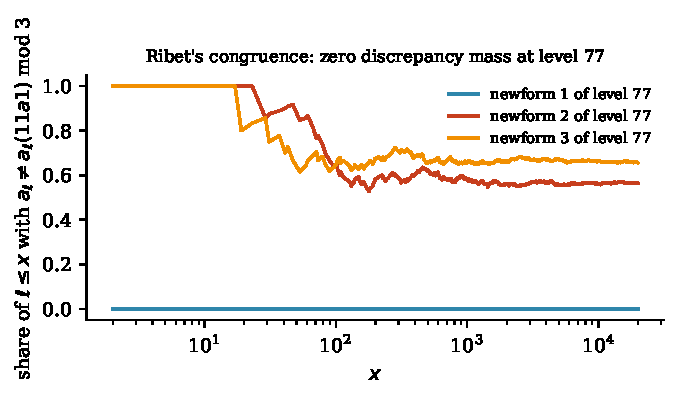
\includegraphics[width=0.72\textwidth]{figs/flt_congruence.pdf}
\caption{Proposition~\ref{prop:fltmodp}: the share of primes $\ell\le x$ at which the coefficients of each rational newform of level $77$ differ modulo $3$ from those of $11a1$. One newform has no discrepancy prime below $2\cdot10^4$, consistent with Ribet's level raising theorem \cite{ribet1984}, which predicts from the condition $a_7(11a1)\equiv-(7+1)\bmod3$ a newform of level $77$ congruent to $11a1$ modulo a prime above $3$.}\label{fig:fltcongruence}
\end{figure}

\begin{theorem}[Fermat's last theorem in Thorin form]\label{thm:fltflt}
Assume Theorems~\ref{thm:fltwiles} and \ref{thm:fltribet} and Mazur's torsion theorem \cite{mazur1977}. Then for every prime $p\ge5$ a solution of $a^p+b^p=c^p$ in nonzero integers would produce a weight two newform $g$ of level dividing $2$ whose mod $p$ discrepancy Thorin mass against the Frey curve is zero. Since $S_2(\Gamma_0(1))=0$ and the Thorin measure of $H_2(\ell)$ is empty (Theorem~\ref{thm:fltempty}), no such $g$ exists, and Fermat's last theorem holds for $p\ge5$.
\end{theorem}

\begin{proof}
The Frey curve $E$ is semistable, hence modular by Theorem~\ref{thm:fltwiles}, with $\bar\rho_{E,p}$ irreducible by Serre's argument from Mazur's torsion theorem \cite{serre1987} (see Proposition~\ref{prop:flteisfrey}), unramified at every odd prime dividing $N_E$ other than $p$, and finite flat at $p$. Apply Theorem~\ref{thm:fltribet} first at $q=p$ if $p\mid N_E$, where $q\not\equiv1\bmod p$ holds trivially, and then one at a time at the odd primes $q\ne p$ of the level, which is now prime to $p$. This gives a newform $g$ of level dividing $2$ and a prime $\mathfrak p'$ above $p$ with $\bar\rho_{g,\mathfrak p'}\cong\bar\rho_{E,p}$ over $\overline{\mathbb F}_p$, which by Proposition~\ref{prop:fltmodp} is the vanishing of the discrepancy Thorin mass. But $S_2(\Gamma_0(1))=0$, and $X_0(2)$ has genus zero, so by Theorem~\ref{thm:fltempty} there are no weight two newforms of level $2$.
\end{proof}

With the exponents $3$ (Euler) and $4$ (Fermat) this gives every $n\ge3$, since each is divisible by $4$ or by an odd prime. So the last line of the proof of Fermat's last theorem, $S_2(\Gamma_0(2))=0$, is elementary, and in the language of this chapter it reads: in characteristic $2$ there is one supersingular elliptic curve, so the isogeny walk is stuck, its Kemeny constant is zero, the Hecke GGC is the zero variable, and its Thorin measure is empty. Equivalently, the Hurwitz quaternions have class number one. Everything before that line is the work of Hellegouarch and Frey (the curve), Frey and Serre (the reduction), Mazur, Ribet, Langlands and Tunnell, Wiles, and Taylor and Wiles (Sections~\ref{sec:fltproof} and \ref{sec:fltweightone}).

\section{Fermat's last theorem, one Thorin measure at a time}\label{sec:fltexplicit}

The previous section answered the title question in outline. This section makes every Thorin measure in the argument explicit: on which space it lives, what it is, which theorem says that it vanishes or does not, and what it is numerically. Two Thorin measures appear. The first, the \emph{Eisenstein Thorin shape} of an elliptic curve, is a single number $c(E,p)\in[0,1]$: the density of the primes $\ell$ with $p\nmid|E(\mathbb F_\ell)|$, which is the local density at $p$ in Koblitz's conjecture \cite{koblitz1988}, in Zywina's form for any image \cite{zywina2011}, read here as the shape of a Gamma law. Mazur's torsion theorem, through Serre's argument, makes it positive for Frey curves when $p\ge5$. The second is the Hecke Thorin measure of Definition~\ref{def:flthecke}, which is empty at level $2$. Given Theorems~\ref{thm:fltwiles} and \ref{thm:fltribet} and Mazur's torsion theorem, a Frey curve, whose shape is positive, would give the second measure an atom; since it has none, there is no Frey curve (Theorem~\ref{thm:flttwo}).

\subsection{The Eisenstein Thorin shape}

The weight two Eisenstein series of prime level $N$ has Hecke eigenvalues $a_\ell=1+\ell$ for $\ell\ne N$. For an elliptic curve the difference from Eisenstein is a point count: $1+\ell-a_\ell(E)=|E(\mathbb F_\ell)|$. So ``$E$ agrees with Eisenstein modulo $p$ at $\ell$'' means exactly that $p$ divides $|E(\mathbb F_\ell)|$.

\begin{definition}\label{def:flteis}
Let $E/\Q$ have conductor $N$ and let $p$ be prime. The \emph{Eisenstein discrepancy} of $(E,p)$ is $Q_{E,p}(\ell)=\mathsf 1\{p\nmid|E(\mathbb F_\ell)|\}$ for primes $\ell\nmid pN$, and its \emph{Eisenstein Thorin shape} is
\[
c(E,p)=\mu_{G_{E,p}}\bigl\{g\in G_{E,p}:\det(1-g)\ne0\bigr\},
\]
where $G_{E,p}\subset\GL_2(\mathbb F_p)$ is the image of $\bar\rho_{E,p}$, with Haar probability measure $\mu_{G_{E,p}}$.
\end{definition}

\begin{proposition}[Gamma law of the Eisenstein discrepancy; (a) this book]\label{prop:flteisgamma}
Let $E/\Q$ be an elliptic curve and $p$ a prime.
\begin{enumerate}
\item[(a)] The Frobenius functional $\Xi_\sigma(Q_{E,p})$ of the zeta random integer converges in law, as $\sigma\downarrow1$, to the Gamma law with shape $c(E,p)$ and scale $1$. Its Thorin measure is $c(E,p)\,\delta_1$, and $c(E,p)$ is the rate at which the prime factors of a random integer hit the primes $\ell$ with $p\nmid|E(\mathbb F_\ell)|$ (Theorem~\ref{thm:hitrate}).
\item[(b)] $c(E,p)=0$ if and only if $\bar\rho_{E,p}^{\mathrm{ss}}\cong1\oplus\chi_p$, with $\chi_p$ the mod $p$ cyclotomic character, if and only if $p$ divides $|E(\mathbb F_\ell)|$ for every $\ell\nmid pN$. In that case $E$ has a rational isogeny of degree $p$. If $E$ is semistable, $c(E,p)=0$ if and only if $\bar\rho_{E,p}$ is reducible.
\item[(c)] If $G_{E,p}=\GL_2(\mathbb F_p)$, then
\[
c(E,p)=c_p:=1-\frac{p^2-2}{(p^2-1)(p-1)},
\]
so that $c_2=\frac13$, $c_3=\frac9{16}$, $c_5=\frac{73}{96}$ and $c_7=\frac{241}{288}$.
\end{enumerate}
\end{proposition}

\begin{proof}
(a) The label of $\ell$ is the conjugacy class of $\bar\rho_{E,p}(\Frob_\ell)$ in the finite group $G_{E,p}$, and $Q_{E,p}(\ell)=1$ exactly when $\det\bigl(1-\bar\rho_{E,p}(\Frob_\ell)\bigr)$, which is $|E(\mathbb F_\ell)|$ modulo $p$, is nonzero. By Chebotarev the labels are equidistributed for Haar measure, and Theorem~\ref{thm:recipggcfun} with $Q\in\{0,1\}$ gives the GGC whose Thorin measure is $\mu(Q=1)\,\delta_1=c(E,p)\,\delta_1$, the Gamma law with shape $c(E,p)$. The hitting rate is Theorem~\ref{thm:hitrate} for the same set of primes.

(b) If $c(E,p)=0$ then every $g\in G_{E,p}$ has eigenvalue $1$, so its characteristic polynomial is $(x-1)(x-\det g)$, which is that of $1\oplus\chi_p$ since $\det\bar\rho_{E,p}=\chi_p$. By Brauer Nesbitt $\bar\rho_{E,p}^{\mathrm{ss}}\cong1\oplus\chi_p$, so $\bar\rho_{E,p}$ is reducible and its invariant line gives a rational $p$ isogeny. The converse and the point count form are immediate. For semistable $E$ the two characters of a reducible $\bar\rho_{E,p}$ are $1$ and $\chi_p$ \cite{serre1972}, so reducibility forces $c(E,p)=0$.

(c) In $\GL_2(\mathbb F_p)$ the elements with eigenvalue $1$ have characteristic polynomial $(x-1)(x-d)$. For each of the $p-2$ values $d\ne0,1$ these form one split semisimple class of size $p(p+1)$; for $d=1$ there are the identity and the $p^2-1$ nontrivial unipotents. The count is $(p-2)p(p+1)+p^2=p^3-2p$, and dividing by $|\GL_2(\mathbb F_p)|=(p^2-1)(p^2-p)$ gives $(p^2-2)/((p^2-1)(p-1))$.
\end{proof}

Part (c) is the class count behind the factor at $p$ of the constant in Koblitz's conjecture on the primality of $|E(\mathbb F_\ell)|$ \cite{koblitz1988,zywina2011}: $c_p/(1-1/p)=1-(p^2-p-1)/((p-1)^3(p+1))$. By a theorem of Katz \cite{katz1981}, the curves with $c(E,p)=0$ in (b) are those isogenous to a curve with a rational point of order $p$. What (a) adds is the reading of this density as the shape of a Gamma law.

So the Eisenstein shape is a Thorin measure with one atom, and the whole content is in the mass of that atom. Two of its behaviours appear in the book's running examples (Figure~\ref{fig:flteis}). For $11a1$ and $p=5$ the shape is exactly $0$: $11a1$ has a rational point of order $5$, so $5$ divides $|11a1(\mathbb F_\ell)|$ for all $664577$ primes $\ell<10^7$ with $\ell\ne5,11$, and the Laplace transform of $\Xi_\sigma(Q)$ is identically $1$. This is Mazur's Eisenstein congruence \cite{mazur1977}: $J_0(11)$ is the curve $11a1$, whose rational torsion, the cuspidal subgroup, has order $5$, the numerator of $(11-1)/12$, and injects into $J_0(11)(\mathbb F_\ell)$ for $\ell\ne11$ (for $\ell\ge3$ by the appendix of \cite{katz1981}, and for $\ell=2$ because its order is odd), so $5$ divides the product $|J_0(11)(\mathbb F_\ell)|$ of the Thorin atoms of $H_{11}(\ell)$. For $37a1$, whose mod $p$ images are all of $\GL_2(\mathbb F_p)$ \cite{serre1972}, the observed shares of discrepancy primes below $10^7$ are $0.3332$, $0.5628$, $0.7611$, $0.8370$, $0.9002$, $0.9178$ for $p=2,3,5,7,11,13$, against $c_p=0.3333$, $0.5625$, $0.7604$, $0.8368$, $0.9008$, $0.9172$, and the Laplace transforms at $\sigma=1.01$ and $\sigma=1.002$ approach $(1+\lambda)^{-c_p}$.

\begin{figure}[t]
\centering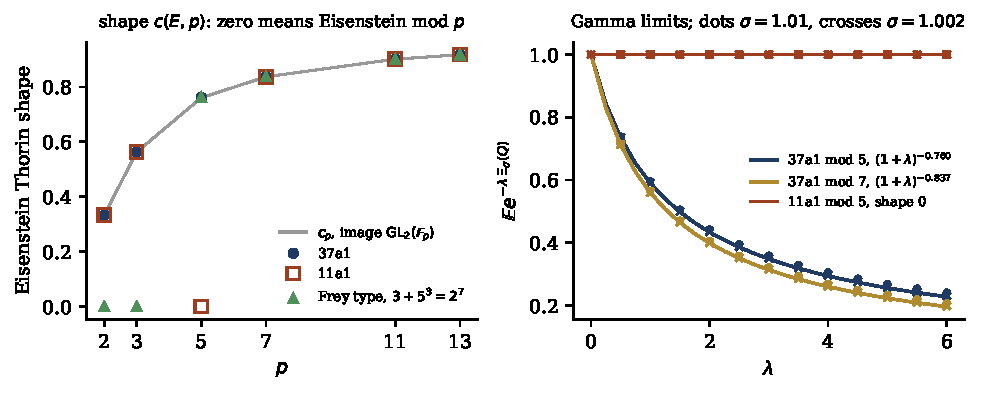
\includegraphics[width=\textwidth]{figs/flt_eisenstein.pdf}
\caption{Proposition~\ref{prop:flteisgamma}. Left: the Eisenstein Thorin shape $c(E,p)$, measured as the share of primes $\ell<10^7$ with $p\nmid|E(\mathbb F_\ell)|$ for $37a1$ and $11a1$, and of primes $\ell<2\cdot10^6$ for the semistable Frey type curve $y^2=x(x+125)(x+128)$ of $3+5^3=2^7$, against $c_p$. Right: Laplace transforms of $\Xi_\sigma(Q_{E,p})$ for $37a1$ modulo $5$ and $7$ and $11a1$ modulo $5$, at $\sigma=1.01$ (dots) and $\sigma=1.002$ (crosses), against the Gamma limits $(1+\lambda)^{-c(E,p)}$.}\label{fig:flteis}
\end{figure}

\subsection{Mazur's theorem and the Eisenstein shape of a Frey curve}

A Frey curve $y^2=x(x-a^p)(x+b^p)$ is semistable and has all its $2$ torsion rational. The second fact gives the Eisenstein shape $c(E,2)=0$, and with Mazur's torsion theorem it gives positive shapes at every $p\ge5$.

\begin{proposition}[Eisenstein shapes of a Frey curve; after Serre \cite{serre1987} and Mazur \cite{mazur1977}]\label{prop:flteisfrey}
Let $E$ be an elliptic curve over $\Q$ with $E[2]\subset E(\Q)$, for example a Frey curve. Then $c(E,2)=0$, and $c(E,p)>0$ for every prime $p\ge5$.
\end{proposition}

\begin{proof}
For odd $\ell$ of good reduction, reduction is injective on $E(\Q)[2]\cong(\Z/2)^2$, so $4$ divides $|E(\mathbb F_\ell)|$ and $Q_{E,2}\equiv0$. If $c(E,p)=0$ for some $p\ge5$, then $\bar\rho_{E,p}^{\mathrm{ss}}\cong1\oplus\chi_p$ by Proposition~\ref{prop:flteisgamma}(b), so $E$, or its quotient $E'$ by the rational subgroup of order $p$, has a rational point of order $p$. An isogeny of odd degree maps $E[2]$ isomorphically onto $E'[2]$, so that curve has rational torsion containing $\Z/2\times\Z/2p$, which Mazur's torsion theorem \cite{mazur1977} excludes for $p\ge5$. This is Serre's argument \cite{serre1987}; see also \cite[Theorem~2.9(c)]{ddt1995}.
\end{proof}

So the irreducibility of $\bar\rho_{E,p}$ for a Frey curve and $p\ge5$, the hypothesis of Ribet's theorem that Serre deduced from Mazur's torsion theorem, reads in Thorin form: the Gamma law of the Eisenstein discrepancy has positive shape; equivalently, $p$ fails to divide $|E(\mathbb F_\ell)|$ for a positive proportion $c(E,p)$ of primes. The hypothesis $p\ge5$ is sharp, and a real Frey type curve shows why. The $abc$ triple $3+5^3=2^7$, written as $-125+128=3$ with $-125\equiv-1\bmod4$ and $32\mid128$, gives the Frey type curve
\[
E_0:\ y^2=x(x+125)(x+128),
\]
which is semistable of conductor $30$ with minimal discriminant $2^63^25^6$. Its shapes, measured over the primes below $2\cdot10^6$, are $c(E_0,2)=0$ and $c(E_0,3)=0$, but $c(E_0,5)=0.762$ and $c(E_0,7)=0.837$, against $c_5=0.760$ and $c_7=0.837$ (Figure~\ref{fig:flteis}, left). At $p=3$ the exponents $6$ and $6$ of the primes $2$ and $5$ are divisible by $3$, so $\bar\rho_{E_0,3}$ is unramified at $2$ and $5$. A genuine Frey curve differs at $2$: there the exponent is $2pv_2(b)-8$, never divisible by an odd $p$, which is why level $2$ remains. And $E_0$ has a rational $3$ isogeny, its Eisenstein shape at $3$ is $0$, and Ribet's theorem, which needs an irreducible $\bar\rho$, does not apply. At $p\ge5$, where Mazur's torsion theorem forces the shape to be positive, the exponents are not divisible by $p$ and there is nothing to lower. A genuine Frey curve would need both at once.

\subsection{The level two Brandt module}

At level $N=2$ the isogeny walk has the single state of Section~\ref{sec:fltoneforms}, and its Brandt matrix is the $1\times1$ matrix $B(\ell)=(\ell+1)$. By Eichler and Gross \cite{eichler1954,eichler1973,gross1987} the constants carry the Eisenstein eigenvalues $\ell+1$, and their orthogonal complement in $L^2$ of the stationary law carries $S_2(\Gamma_0(2))$, which is $0$ here. So every weight two Hecke eigensystem of level $2$, cuspidal or not, is visible on this one point space, and a mod $p$ eigensystem there could be of two kinds, of which only the first occurs:
\begin{enumerate}
\item[(E)] the Eisenstein system $a_\ell=\ell+1$ of the stationary law, against which a curve $E$ has discrepancy Thorin shape $c(E,p)$;
\item[(C)] a cuspidal system, an atom of the Hecke Thorin measure of $H_2(\ell)$, which is empty by Theorem~\ref{thm:fltempty}.
\end{enumerate}

\begin{theorem}[Fermat's last theorem as two Thorin statements]\label{thm:flttwo}
Assume Theorems~\ref{thm:fltwiles} and \ref{thm:fltribet} and Mazur's torsion theorem \cite{mazur1977}, used through Proposition~\ref{prop:flteisfrey}. Let $p\ge5$ and suppose $a^p+b^p=c^p$ with $abc\ne0$, and let $E$ be its Frey curve. Then $\bar\rho_{E,p}$ would have zero discrepancy Thorin mass against some weight two eigensystem of level $2$. But:
\begin{enumerate}
\item[(i)] against the Eisenstein system the discrepancy is the Gamma law of shape $c(E,p)>0$ (Propositions~\ref{prop:flteisgamma} and \ref{prop:flteisfrey});
\item[(ii)] there is no cuspidal system, because the Hecke Thorin measure of level $2$ is empty (Theorem~\ref{thm:fltempty}).
\end{enumerate}
Hence there is no such solution.
\end{theorem}

\begin{proof}
By Proposition~\ref{prop:flteisfrey}, $c(E,p)>0$, so $\bar\rho_{E,p}$ is irreducible by Proposition~\ref{prop:flteisgamma}(b), since $E$ is semistable. It is unramified at the odd primes $q\ne p$ dividing $N_E$ and finite flat at $p$ (Section~\ref{sec:fltproof}). By Theorem~\ref{thm:fltwiles} it comes from a newform of level $N_E$, and Theorem~\ref{thm:fltribet}, applied in the order of the proof of Theorem~\ref{thm:fltflt}, gives a newform $g$ of level dividing $2$, hence of level $2$ since $S_2(\Gamma_0(1))=0$, and a prime $\mathfrak p'$ above $p$ with $\bar\rho_{g,\mathfrak p'}\cong\bar\rho_{E,p}$ over $\overline{\mathbb F}_p$, that is (Proposition~\ref{prop:fltmodp}) zero discrepancy Thorin mass between $E$ and a cuspidal system of level $2$. This contradicts (ii). Statement (i) shows that the Eisenstein system cannot take its place: it is the same positivity that made Ribet's theorem applicable.
\end{proof}

The theorem uses two Thorin measures in opposite directions. The Eisenstein shape of the Frey curve must be \emph{positive}, a statement about Frobenius statistics that follows, by Serre's argument, from Mazur's theorem on rational torsion, proved through the Eisenstein ideal; the Hecke Thorin measure of level $2$ must be \emph{empty}, a statement about the one state isogeny walk that is equivalent to the class number one of the Hurwitz quaternions. Modularity (Wiles; Taylor and Wiles) and Ribet's theorem connect the two by transporting the Frobenius labels of the Frey curve, with zero discrepancy mass, from level $N_E$ to level $2$.

\subsection{The proof of Fermat's last theorem, step by step}

\begin{center}\small
\begin{tabular}{@{}p{0.27\textwidth}p{0.47\textwidth}p{0.18\textwidth}@{}}
\toprule
\raggedright Step & \raggedright Probabilistic or Thorin form & \raggedright Status\tabularnewline
\midrule
\raggedright Langlands Tunnell, weight one & \raggedright zero discrepancy Thorin mass between the Artin representation and a weight one form (Theorem~\ref{thm:recipthorin}(a)); both have the atomic label law of Proposition~\ref{prop:fltatomic}, which does not produce the form (Corollary~\ref{cor:reciplaw}) & \raggedright theorem (Langlands, Tunnell)\tabularnewline
\raggedright mod $3$ to weight two & \raggedright Wilton type congruence, zero discrepancy mass & \raggedright theorem (Wiles)\tabularnewline
\raggedright modularity of semistable curves & \raggedright reflection symmetry of twisted P\'olya kernels & \raggedright theorem (Wiles; Taylor and Wiles)\tabularnewline
\raggedright Frey curve (Hellegouarch, Frey), full $2$ torsion & \raggedright implies Eisenstein shape $c(E,2)=0$ (Proposition~\ref{prop:flteisfrey}) & \raggedright elementary\tabularnewline
\raggedright irreducibility of $\bar\rho_{E,p}$, $p\ge5$ & \raggedright Eisenstein shape $c(E,p)>0$: Gamma law of the discrepancy, positive hitting rate & \raggedright theorem (Mazur; Serre)\tabularnewline
\raggedright Ribet's level lowering & \raggedright zero mod $p$ discrepancy Thorin mass against a newform of level dividing $N/q$, zero hitting rate & \raggedright theorem (Ribet)\tabularnewline
\raggedright $g(X_0(2))=0$ & \raggedright empty Hecke Thorin measure, Kemeny constant $0$; only the Eisenstein system lives at level $2$ & \raggedright elementary\tabularnewline
\bottomrule
\end{tabular}
\end{center}

The table shows what the Thorin framework restates. It restates the last four steps as statements about positive measures, Gamma shapes and hitting times, and modularity as a symmetry in law that can be tested numerically, though not verified, from point counts and the conductor. The Thorin form of the analytic theory of $L(s,E)$, complete monotonicity of the heat trace, is GRH, which Fermat's last theorem does not need and which remains open.

\subsection{Where probability meets the deep part}

Two points of the argument of Wiles and of Taylor and Wiles have a direct probabilistic reading. The Taylor Wiles method needs, for each $n$, auxiliary primes $q\equiv1\bmod p^n$ at which $\bar\rho(\Frob_q)$ has distinct eigenvalues; their existence, with positive density, once $\bar\rho$ is absolutely irreducible on the absolute Galois group of $\Q(\sqrt{p^*})$, where $p^*=(-1)^{(p-1)/2}p$, is a Chebotarev statement, which by Theorem~\ref{thm:hitrate} is a positive hitting rate of a class by the prime factors of a random integer. And the modularity of the Frey curve itself, if one wanted it in the probabilistic forms of Chapter~\ref{ch:recip}, is the reflection symmetry of the twisted P\'olya kernels required by Weil's converse theorem. A Thorin converse theorem of the kind proved at level one in Corollary~\ref{cor:recipconverse}, not known at level $N$ (Open Problem~\ref{op:recipgln}), would take as its hypothesis a positivity statement that contains GRH for $L(s,E)$, which is open; without GRH it could give neither modularity nor GRH. The Thorin framework restates modularity; it does not supply it.

\subsection{Open problems}

\begin{problem}[Hasse Weil from hitting times]\label{op:flthasse}
Give a probabilistic proof of the bound $|a_\ell(f)|\le2\sqrt\ell$ of Eichler and Shimura with Weil for weight two newforms of prime level $N$, for instance through hitting times or a heat kernel on the supersingular isogeny graph. The positivity of the Thorin atoms of $H_N(\ell)$ needs only $a_\ell(f)<\ell+1$, which Perron Frobenius gives; the bound itself gives the estimates of Corollary~\ref{cor:hithasse}, and its local Thorin form is that of Chapter~\ref{ch:10c}. Compare Open Problem~\ref{op:rp}, where no geometric proof is available.
\end{problem}

\begin{problem}[Patching as a Gamma process]\label{op:fltpatch}
The Taylor Wiles method chooses, for each $n$, finite sets of auxiliary primes $q\equiv1\bmod p^n$ at which $\bar\rho(\Frob_q)$ has distinct eigenvalues; by Chebotarev and Theorem~\ref{thm:hitrate} such primes occur among the large prime factors of a zeta random integer at a positive rate. Is there a formulation of the patching argument in which the auxiliary sets are the atoms of the Gamma process of Section~\ref{sec:recipgammaproc} in a fixed Chebotarev class, and the patched objects are limits in law as $\sigma\downarrow1$?
\end{problem}

\begin{problem}[A probabilistic Mazur theorem]\label{op:fltmazur}
Proposition~\ref{prop:flteisfrey} deduces $c(E,p)>0$ for $p\ge5$ and every curve with $E[2]\subset E(\Q)$ from Mazur's torsion theorem. One rational point of order $2$ is not enough: the semistable curve $y^2+xy=x^3-45x+81$ of conductor $66$ has torsion $\Z/10$, so $c(E,5)=0$. Is there a proof of Proposition~\ref{prop:flteisfrey} through the Gamma law of the Eisenstein discrepancy and the isogeny walks of Chapter~\ref{ch:hit}? Such a proof must use an input special to $\Q$: over some quadratic fields there are curves with torsion $\Z/2\times\Z/10$ \cite{kenkumomose1988,kamienny1992,kamiennynajman2012}, whose analogue of the Eisenstein shape at $5$, over the primes of the field, vanishes.
\end{problem}

\section{Notes}

The curve goes back to Hellegouarch and Frey \cite{hellegouarch1975,frey1986}, and the reduction of Fermat's last theorem to modularity is due to Frey and Serre \cite{frey1986,serre1987}, with level lowering by Ribet \cite{ribet1990}, and the modularity of semistable curves to Wiles and to Taylor and Wiles \cite{wiles1995,taylorwiles1995}; Darmon, Diamond and Taylor \cite{ddt1995} give a detailed account, including the use of Langlands and Tunnell \cite{langlands1980,tunnell1981} and the $3$ to $5$ switch. Mazur's theorems on rational torsion and on rational isogenies of prime degree are in \cite{mazur1977,mazur1978}; Serre deduced from the first the irreducibility of $\bar\rho_{E,p}$ for Frey curves and $p\ge5$ \cite{serre1987}, which Proposition~\ref{prop:flteisfrey} restates as a positive shape. Level raising is due to Ribet \cite{ribet1984,ribet1990b}, and the removal of semistability to Breuil, Conrad, Diamond and Taylor \cite{bcdt2001}. Deligne and Serre \cite{deligneserre1974} attach an odd irreducible two dimensional Artin representation to each weight one newform, and by Khare and Wintenberger, with Kisin \cite{kharewintenberger2009,kharewintenberger2009b,kisin2009}, every such representation arises in this way. The label law does not see parity: the $S_3$ representations of the splitting fields of $x^3-x-1$ (odd) and of $x^3-4x-1$ (even) have the same label law; for the even representations see Open Problem~\ref{op:reciplaw} and Problem~\ref{cp:recipicosa}. Wilton's congruence is \cite{wilton1930}, and Serre \cite{serre1968b} explained it by the mod $23$ representation of $\Delta$ (see also Swinnerton Dyer \cite{swinnertondyer1973}). Supersingular curves and their endomorphism rings go back to Deuring \cite{deuring1941}; quaternion orders and Brandt matrices are in Eichler and Gross \cite{eichler1954,eichler1973,gross1987}.

The P\'olya kernel is P\'olya's (Chapter~\ref{ch:10}), in the form of Chapter~\ref{ch:recip}, from which the Frobenius functionals, the Galois heat trace and the Thorin converse theorem also come; the Rankin Selberg density $U_\alpha$ is the density $U_{\mathrm{ar}}$ of Chapter~\ref{ch:10d}, Proposition~\ref{prop:fltwald} is the case $\eta(z)^2\eta(11z)^2$ of Theorem~\ref{thm:10dvdp}, and the Kemeny constant, hitting rates and explosion times are from Chapter~\ref{ch:hit}. The density $c(E,p)$ of Definition~\ref{def:flteis} is classical: it is the local density at $p$ in Koblitz's conjecture \cite{koblitz1988} that, for a curve without complex multiplication and not isogenous to one with a rational torsion point, the number of primes $\ell\le x$ for which $|E(\mathbb F_\ell)|$ is prime is asymptotic to a constant times $x/(\log x)^2$; Zywina \cite{zywina2011} built the constant from the Haar measures of the images of $E$ modulo all integers, which corrects for their entanglement, and no case with a positive constant is known. The vanishing of $c(E,p)$ is characterised by Katz \cite{katz1981} and, for semistable curves, by Serre \cite{serre1972}. New here are the readings of these statements as Thorin statements (Definition~\ref{def:flteis}, Proposition~\ref{prop:flteisgamma}(a) and Theorem~\ref{thm:flttwo}) and the numerical checks; Propositions~\ref{prop:fltsymmetric}, \ref{prop:fltwald} and \ref{prop:fltmodp} and Theorems~\ref{thm:fltempty} and \ref{thm:fltflt} are restatements in this book's language, and Proposition~\ref{prop:fltatomic} combines Deligne and Serre with the Sato Tate theorem.

\section{Exercises}

\begin{enumerate}
\item Show that $H_{11}(\ell)$ is exponential with rate $|11a1(\mathbb F_\ell)|$, and check that $\E H_{11}(2)=\frac15$ agrees with $K_{11}(2)=\frac35$ of Chapter~\ref{ch:hit}.
\item Verify Wilton's congruence for $p<1000$ by computing $\tau(p)$ from $\Delta=q\prod(1-q^n)^{24}$ and the number of roots of $x^3-x-1$ modulo $p$.
\item Prove from the Laplace pair $\int_0^\infty\log(1+b^2/y^2)\cos(ay)\,dy=\frac\pi a(1-e^{-ab})$ that\[\int_0^\infty\log\Bigl(1+\frac sz\Bigr)U_\alpha(z)\,dz=-\sqrt s\,\frac{D'}D(\alpha)-\log D(\alpha)+\log D(\alpha+\sqrt s).\]Compare Lemma~\ref{lem:10dsin2}, which proves it by another route.
\item Count the elements of $\GL_2(\mathbb F_p)$ without eigenvalue $1$ for $p=3,5,7$ by machine and check $c_p$ of Proposition~\ref{prop:flteisgamma}. Show that $c_p=1-\frac1p+O(p^{-2})$, so that, for a curve with image $\GL_2(\mathbb F_p)$ and large $p$, almost every prime is an Eisenstein discrepancy prime.
\item For $E_0:y^2=x(x+125)(x+128)$ find the rational $3$ isogeny, and show that $3$ divides $|E_0(\mathbb F_\ell)|$ for every $\ell\ge7$.
\item Count the Hurwitz quaternions of norm $n\le20$ by enumeration and compare with $24\sum_{d\mid n,\,d\text{ odd}}d$. Explain why the formula fails for the Lipschitz quaternions $a+bi+cj+dk$ with $a,b,c,d\in\Z$.
\item For $37a1$ show that $\Phi_E$ is odd and compute $\int_0^\infty u\,\Phi_E(u)\,du$ numerically; relate it to $\Lambda'(1,E)$ and hence to the Birch and Swinnerton Dyer leading term.
\end{enumerate}

\section{Open computational problems}

\begin{compproblem}[Explosion cumulants of elliptic curves]\label{cp:fltheat}
Objective: for elliptic curves of both root numbers, compute $\int_0^\infty x^{m-1}\bigl(\mathcal W_E(x)-\frac r2\bigr)\,dx$ for $m=1,2,3$, with $r$ the order of vanishing at the centre, from the point counts, the conductor and the gamma factor through Definition~\ref{def:recipheat}, as Section~\ref{sec:fltthorinec} does for $11a1$. If GRH holds for $L(s,E)$, which is not known, these are $(m-1)!\sum_{\gamma>0}\gamma^{-2m}$, and for $r=0$ they are the first three cumulants of the explosion time $T_E$ (Theorem~\ref{thm:hitexplosion}). Objects and scale: one curve from each isogeny class of conductor below $10^3$, which includes curves of rank $0$, $1$ and $2$; prime powers up to $10^8$. Route: \texttt{thorin\_ec.py}, with point counts from the pipeline of Chapter~\ref{ch:05} or from \texttt{ellap}; ball arithmetic for the archimedean term and on the range of $x$ that the primes control, as in Problem~\ref{cp:hitexplosion}; beyond it, the sum over the zeros located by \texttt{lfunzeros}; $r$ from \texttt{ellanalyticrank}. Deliverable: a table by conductor, root number and rank of the integrals over the controlled range, with rigorous error bounds, against the same integrals over the zeros, and of the full integrals against the power sums $S_1$, $S_2$, $S_3$ of \eqref{eq:10bkS} computed from central Taylor coefficients as in Chapter~\ref{ch:10b}. Why it matters: it is the family version of Problem~\ref{cp:hitexplosion}, and it covers the curves with a central zero, which the problem on monotonicity across weights and levels in Chapter~\ref{ch:10} leaves out; a disagreement beyond the error bounds would point to a zero off the line or to an error in the data, while agreement does not verify GRH.
\end{compproblem}

\begin{compproblem}[Koblitz's conjecture and Eisenstein shapes]\label{cp:flteis}
Objective: measure the Eisenstein shapes $c(E,p)$ of Definition~\ref{def:flteis} for $p\le37$ and the number of primes $\ell\le X$ for which $|E(\mathbb F_\ell)|$ is prime, and compare the counts with Koblitz's conjecture \cite{koblitz1988} in the form refined by Zywina \cite{zywina2011}, whose constant is built from the same Haar measures as the shapes, corrected for the entanglement of the images modulo different primes. Objects and scale: about $20$ curves with different images, among them $37a1$, whose mod $p$ images are all of $\GL_2(\mathbb F_p)$, curves with a rational isogeny of degree $2$, $3$, $5$ or $7$ but no rational point of that order, $11a1$ and the curve $E_0$ of Section~\ref{sec:fltexplicit}, whose constants vanish, and one curve with complex multiplication; primes $\ell\le10^{10}$. Route: point counts from the pipeline of Chapter~\ref{ch:05}; the images from the LMFDB \cite{lmfdb} and the classifications of \cite{rszb2022,zywina2022}; $c(E,p)$ by counting the elements of the image without eigenvalue $1$; the Laplace transforms of $\Xi_\sigma(Q_{E,p})$ against $(1+\lambda)^{-c(E,p)}$ with $\sigma-1\ge5/\log X$, as in Problem~\ref{cp:recipgamma}. Deliverable: for each curve the constant, the counts against the prediction with normalised fluctuations, and the measured shapes and hitting rates against their Haar values. Why it matters: the shapes give the local factors of Koblitz's constant, so the Gamma laws of Proposition~\ref{prop:flteisgamma} meet a conjecture that is open for every curve with a positive constant; Problem~\ref{cp:05lt} tests the Lang Trotter constants, which are built from the same images.
\end{compproblem}

\begin{compproblem}[Level raising congruences]\label{cp:fltlevel}
Objective: test Proposition~\ref{prop:fltmodp} and Ribet's level raising condition \cite{ribet1984} at scale. For each rational newform $g$ of weight two and level $M$ and each prime $p$ with $\bar\rho_{g,p}$ irreducible, list the primes $q\nmid Mp$ with $a_q(g)\equiv\pm(q+1)\bmod p$, find the newforms $f$ of level dividing $Mq$ and divisible by $q$ whose coefficients are congruent to those of $g$ modulo a prime above $p$, and compute the discrepancy masses of all pairs $(g,f)$. Objects and scale: rational newforms of level $M\le200$, $p\in\{3,5,7\}$, primes $q<50$, so levels below $10^4$. Route: Hecke eigenvalues from the LMFDB \cite{lmfdb} or from modular symbols (\texttt{mfinit} in PARI/GP, or Sage); congruences proved by comparing coefficients up to the Sturm bound; discrepancy masses from the joint mod $p$ Frobenius classes, as in Figure~\ref{fig:fltcongruence}, against their Chebotarev values computed from the images. Deliverable: a table of the predicted congruences against those found, with the residue fields and the coefficient fields of $f$, and the distribution of the discrepancy masses of the noncongruent pairs. Why it matters: the chapter shows one congruence, between $11a1$ and a newform of level $77$; Ribet's theorem \cite{ribet1984,ribet1990b} predicts all of them, and the masses of the noncongruent pairs show how far apart in law distinct mod $p$ representations are, the mod $p$ counterpart of the problem on near coincidences of newforms in Chapter~\ref{ch:01} and of the pairs of curves of Problem~\ref{cp:recipgammaproc}.
\end{compproblem}
